\documentclass[12pt,compress,ngerman,utf8,t]{beamer}
\usepackage{etex}
\usepackage[ngerman]{babel}
\usepackage{calc,dashrule,tabto,tikz}
\usetikzlibrary{arrows}
\usepackage[protrusion=true,expansion=true]{microtype}
\usepackage[normalem]{ulem}

\graphicspath{{images/}}

\title[Mathematische Alternativuniversen]{Mathematische Alternativuniversen}
\author[Ingo Blechschmidt]{\textcolor{white}{Ingo Blechschmidt}} % \\ \scriptsize Lehrstuhl für Algebra und Zahlentheorie an der Universität Augsburg \\}}
\date[2017-01-13]{\vspace*{-4em}\ \\\textcolor{white}{\scriptsize Forschungskolloquium der Augsburger Stipendiatengruppe \\ 13. Januar 2017}}

\useinnertheme[shadow=true]{rounded}
\useoutertheme{split}
\usecolortheme{orchid}
\usecolortheme{whale}
\setbeamerfont{block title}{size={}}

\useinnertheme{rectangles}

\usecolortheme{seahorse}
\definecolor{mypurple}{RGB}{150,0,255}
\setbeamercolor{structure}{fg=mypurple}
\definecolor{myred}{RGB}{150,0,0}
\setbeamercolor*{title}{bg=myred,fg=white}
\setbeamercolor*{titlelike}{bg=myred,fg=white}

\usefonttheme{serif}
\usepackage[T1]{fontenc}
\usepackage{libertine}

\setbeamertemplate{navigation symbols}{}

\setbeamertemplate{title page}[default][colsep=-1bp,rounded=false,shadow=false]
\setbeamertemplate{frametitle}[default][colsep=-2bp,rounded=false,shadow=false,center]

\newcommand{\hil}[1]{{\usebeamercolor[fg]{item}{\textbf{#1}}}}
\setbeamertemplate{frametitle}{%
  \vskip1em%
  \leavevmode%
  \begin{beamercolorbox}[dp=1ex,center]{}%
      \usebeamercolor[fg]{item}{\textbf{\textsf{\Large \insertframetitle}}}
  \end{beamercolorbox}%
}

\setbeamertemplate{footline}{%
  \leavevmode%
  \hfill%
  \begin{beamercolorbox}[ht=2.25ex,dp=1ex,right]{}%
    \usebeamerfont{date in head/foot}
    \insertframenumber\,/\,\inserttotalframenumber\hspace*{1ex}
  \end{beamercolorbox}%
  \vskip0pt%
}

\begin{document}

% http://www.ufointernationalproject.com/wp-content/uploads/2015/11/a23.jpg
{\usebackgroundtemplate{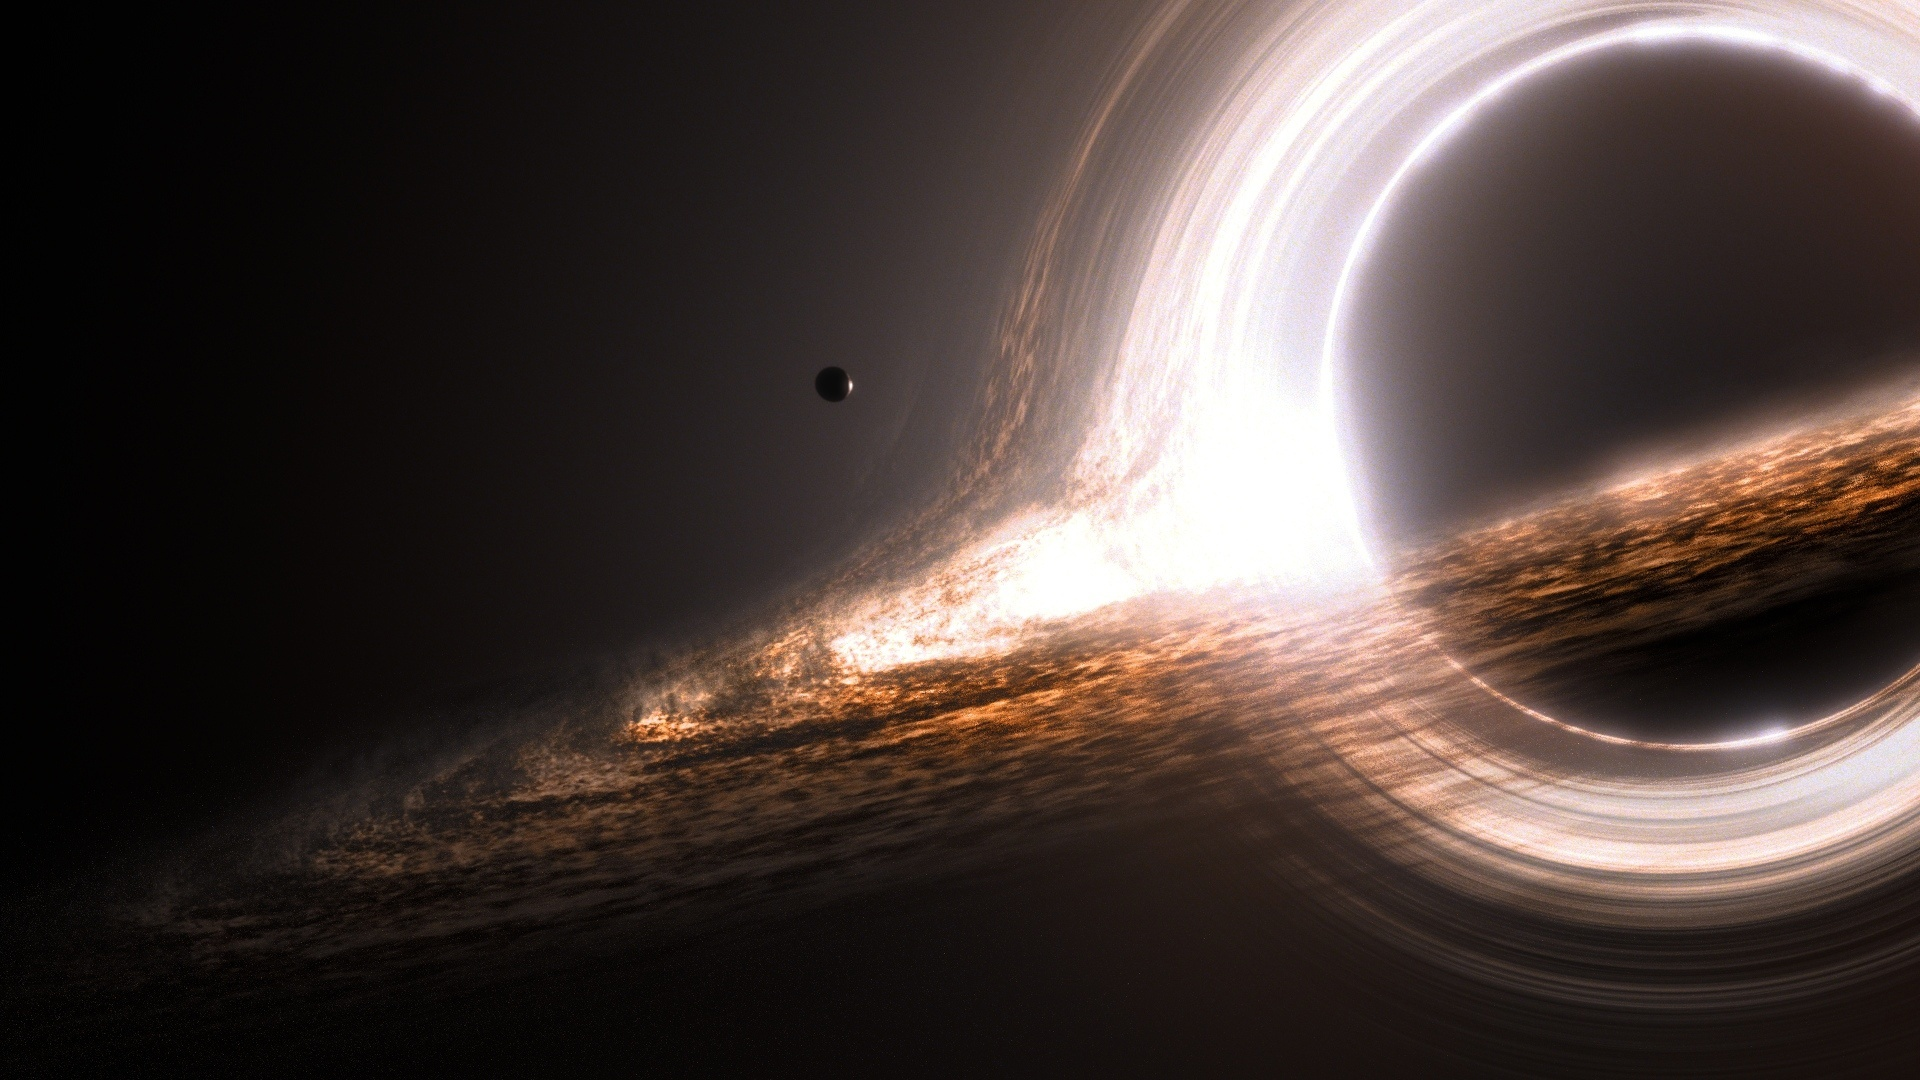
\includegraphics[height=\paperheight]{images/interstellar}}
\frame{\vspace*{12em}\titlepage}}
\frame{\tableofcontents}

\section{Über Wahrheit}

\begin{frame}{Über Wahrheit}
  \vspace*{-0.5em}
  \begin{columns}[t]
    \begin{column}{0.32\textwidth}
      \centering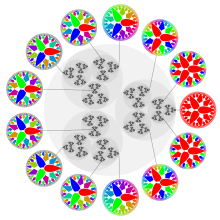
\includegraphics[width=0.7\textwidth]{p-adic-numbers}
      \medskip

      "`Es gibt unendlich viele Primzahlen."'
    \end{column}
    \begin{column}{0.32\textwidth}
      \centering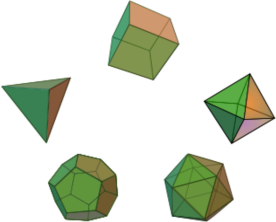
\includegraphics[width=0.9\textwidth]{platonic-solids}
      \medskip

      "`Es gibt nur fünf platonische Körper."'
    \end{column}
    \begin{column}{0.37\textwidth}
      \centering
\includegraphics[width=0.7\textwidth]{hafez-tomb}
      \medskip

      "`Der goldene Schnitt ist die irrationalste Zahl."'
    \end{column}
  \end{columns}
  \bigskip

  \begin{itemize}
    \item Mathematische Aussagen werden als völlig objektiv und
    unabhängig von menschlichen Stimmungen angesehen.
    \pause
    \item Tatsächlich hängt ihr Wahrheitsgehalt aber von der Wahl des
    \hil{mathematischen Universums} ab:
    \begin{enumerate}
      \item Die üblichen Axiome legen das Spiel nicht eindeutig fest.
      \item Wir können die Axiome auch modifizieren.
    \end{enumerate}
  \end{itemize}
\end{frame}


\section[Kontinuumshypothese]{Fallbeispiel: die Kontinuumshypothese}

\subsection[Ganze Zahlen]{Wie viele ganze Zahlen gibt es?}

\begin{frame}{Größenvergleiche im Unendlichen}
  \begin{center}
    \begin{tikzpicture}
    \draw[latex-latex] (-3.5,0) -- (3.5,0);
    \foreach \x in {-3,-2,-1,0,1,2,3}
    \draw[shift={(\x,0)},color=black] (0pt,3pt) -- (0pt,-3pt);
    \foreach \x in {-3,-2,-1,0,1,2,3}
    \draw[shift={(\x,0)},color=black] (0pt,0pt) -- (0pt,-3pt) node[below] {$\x$};
    \end{tikzpicture}
  \end{center}

  Welche Zahlenmenge ist größer?
  \medskip

  \begin{itemize}
    \item die Menge der natürlichen Zahlen: \tabto{6.1cm}$0,\ 1,\ 2,\ \ldots$
    \item die Menge der ganzen Zahlen: \tabto{6.1cm}$\ldots,\ -2,\ -1,\ 0,\ 1,\ 2,\ \ldots$
  \end{itemize}
  \pause
  \bigskip

  \centering
  
\includegraphics[height=0.3\textheight]{spielzeughaufen-1}
  \qquad
  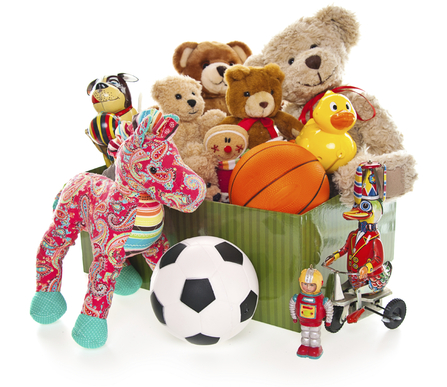
\includegraphics[height=0.3\textheight]{spielzeughaufen-2}
  \par
\end{frame}

\newcommand{\rr}{$\quad\longleftrightarrow\quad$}
\begin{frame}{Größenvergleiche im Unendlichen}
  Sie sind \hil{gleich groß}.
  \bigskip

  \centering
  \begin{tabular}{ccc}
    \uline{\quad alle nat. Zahlen \quad} && \uline{\quad alle ganzen Zahlen \quad} \\
    $0$ & \rr & $\phantom{+}0$ \\
    $1$ & \rr & $\phantom{+}1$ \\
    $2$ & \rr & $-1$ \\
    $3$ & \rr & $\phantom{+}2$ \\
    $4$ & \rr & $-2$ \\
    $5$ & \rr & $\phantom{+}3$ \\
    $6$ & \rr & $-3$ \\
    $\vdots$ && $\vdots$
  \end{tabular}
  \par
\end{frame}


\subsection[Reelle Zahlen]{Wie viele reelle Zahlen gibt es?}


\newcommand{\marked}[1]{\framebox{#1}}
\newcommand{\unmarked}[1]{\textcolor{white}{\framebox{\textcolor{black}{#1}}}}

\begin{frame}{Wie viele reelle Zahlen gibt es?}
  Welche Zahlenmenge ist größer?

  \begin{itemize}
    \item die Menge der natürlichen Zahlen: \tabto{6.1cm}$0,\ 1,\ 2,\ \ldots$
    \item die Menge der reellen Zahlen: \tabto{6.1cm}$0{,}25,\ \tfrac{1}{3},\ \pi,\ \sqrt{2},\ \ldots$
  \end{itemize}
  \pause

  \hil{Es gibt mehr reelle Zahlen als natürliche.}
  \pause
  \bigskip

  \centering
  \only<3>{\begin{tabular}{ccc}
    \uline{\quad alle nat. Zahlen \quad} && \uline{\quad alle reellen Zahlen \quad} \\
    $0$ & \rr & $\unmarked{0}{,}\unmarked{2}\unmarked{5}\unmarked{0}\unmarked{0}\unmarked{0}\unmarked{0}\ldots$ \\
    $1$ & \rr & $\unmarked{3}{,}\unmarked{1}\unmarked{4}\unmarked{1}\unmarked{5}\unmarked{9}\unmarked{2}\ldots$ \\
    $2$ & \rr & $\unmarked{1}{,}\unmarked{4}\unmarked{1}\unmarked{4}\unmarked{2}\unmarked{1}\unmarked{3}\ldots$ \\
    $3$ & \rr & $\unmarked{1}{,}\unmarked{2}\unmarked{3}\unmarked{4}\unmarked{5}\unmarked{6}\unmarked{7}\ldots$ \\
    $\vdots$ && $\vdots$
  \end{tabular}}%
  \only<4->{\begin{tabular}{ccc}
    \uline{\quad alle nat. Zahlen \quad} && \uline{\quad alle reellen Zahlen \quad} \\
    $0$ & \rr & $\marked{0}{,}\unmarked{2}\unmarked{5}\unmarked{0}\unmarked{0}\unmarked{0}\unmarked{0}\ldots$ \\
    $1$ & \rr & $\unmarked{3}{,}\marked{1}\unmarked{4}\unmarked{1}\unmarked{5}\unmarked{9}\unmarked{2}\ldots$ \\
    $2$ & \rr & $\unmarked{1}{,}\unmarked{4}\marked{1}\unmarked{4}\unmarked{2}\unmarked{1}\unmarked{3}\ldots$ \\
    $3$ & \rr & $\unmarked{1}{,}\unmarked{2}\unmarked{3}\marked{4}\unmarked{5}\unmarked{6}\unmarked{7}\ldots$ \\
    $\vdots$ && $\vdots$
  \end{tabular}}

  \only<5>{Was ist mit $1{,}225\ldots$?}
  \par
\end{frame}


\subsection[Zwischenstufe]{Gibt es eine Zwischenstufe?}

\begin{frame}{Die Kontinuumshypothese}
  \begin{columns}[t]
    \begin{column}{0.34\textwidth}
      \centering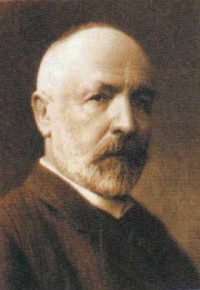
\includegraphics[height=0.5\textheight]{georg-cantor} \\
      {\scriptsize Georg Cantor (* 1845, † 1918)\par}
      \bigskip

      Gibt es eine Zwischenstufe zwischen $\mathbb{N}$ und $\mathbb{R}$?
    \end{column}
    \pause

    \begin{column}{0.34\textwidth}
      \centering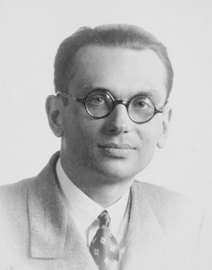
\includegraphics[height=0.5\textheight]{kurt-goedel} \\
      {\scriptsize Kurt Gödel (* 1906, † 1978)\par}
      \bigskip

      Es gibt keinen Beweis, dass es eine Zwischenstufe gibt.
    \end{column}
    \pause

    \begin{column}{0.34\textwidth}
      \centering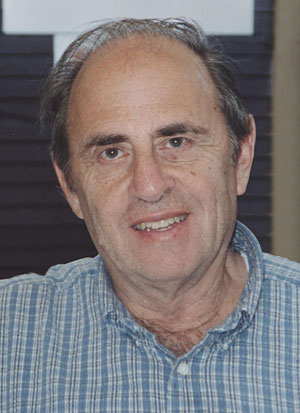
\includegraphics[height=0.5\textheight]{paul-cohen} \\
      {\scriptsize Paul Cohen (* 1934, † 2007)\par}
      \bigskip

      Es gibt keinen Beweis, dass es keine Zwischenstufe gibt.
    \end{column}
  \end{columns}
\end{frame}


\section[Beispiele]{Beispiele für Alternativuniversen}

% \begin{document}

\begin{frame}{Beispiele für Alternativuniversen}
  \centering
  In \hil{Gödels Topos} gilt: \\
  Es gibt keine Zwischenstufe zwischen $\mathbb{N}$ und $\mathbb{R}$.
  \bigskip

  In \hil{Cohens Topos} gilt: \\
  Es gibt eine Zwischenstufe zwischen $\mathbb{N}$ und $\mathbb{R}$.

  {\usebeamercolor[fg]{item}\hdashrule{\textwidth}{1pt}{3mm}\medskip}

  \pause

  Im \hil{glatten Topos} gilt: \\
  Es gibt infinitesimale Zahlen $\varepsilon$ mit $\varepsilon^2 = 0$, aber $\varepsilon \neq 0$.
  \bigskip

  \only<2>{
    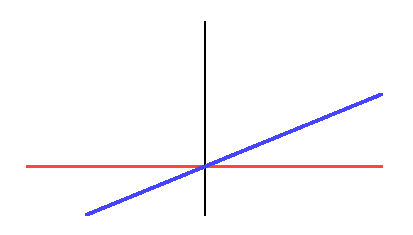
\includegraphics[height=0.3\textheight]{sdg-schnittverhalten1}
    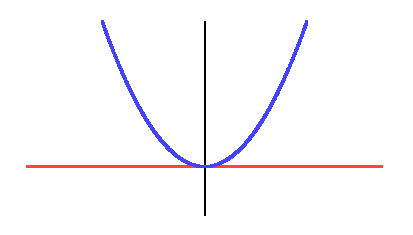
\includegraphics[height=0.3\textheight]{sdg-schnittverhalten2}
  }\pause

  Im \hil{effektiven Topos} gilt: \\
  Jede Funktion $\mathbb{N} \to \mathbb{N}$ ist durch ein Programm berechenbar.
  \bigskip
  \pause

  Im \hil{Zariski-Topos} gilt: \\
  Jede Funktion $\mathbb{R} \to \mathbb{R}$ ist ein Polynom.
  \bigskip
  \par
\end{frame}


\section[Motivation]{Motivation fürs Studium von Alternativuniversen}

% \begin{document}

{\usebackgroundtemplate{\begin{minipage}{\paperwidth}\vspace*{4.95cm}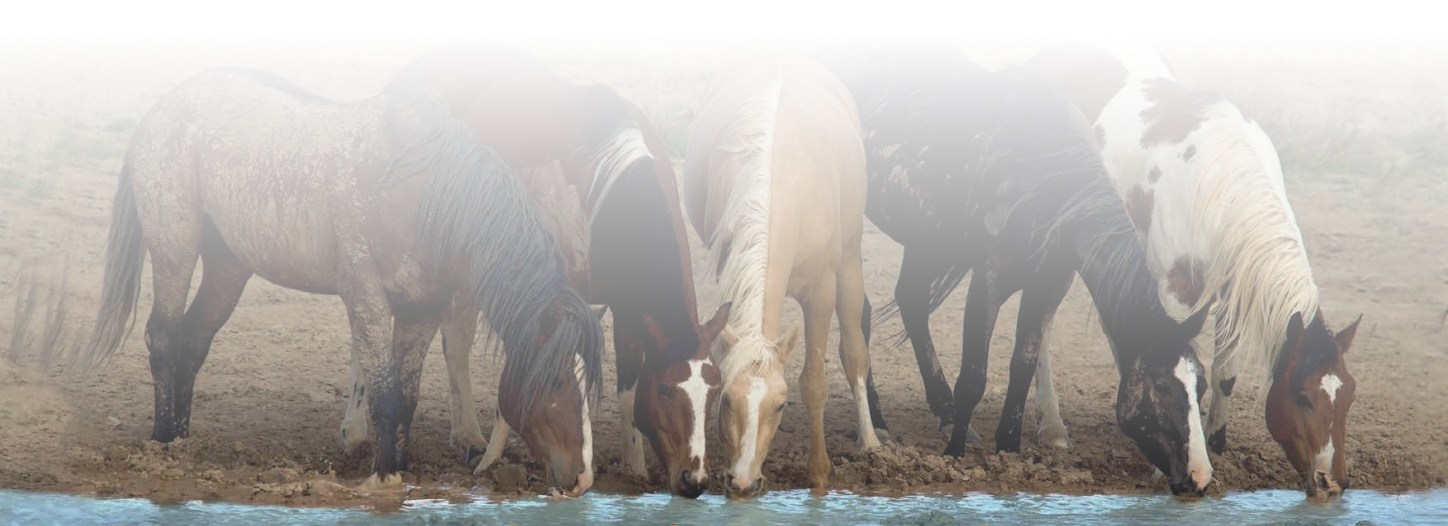
\includegraphics[width=\paperwidth]{topos-horses}\end{minipage}}
\begin{frame}{Wieso sich mit Topoi befassen?}
  Weil sie \ldots
  \begin{itemize}
    \item existieren,
    \item einen Beitrag zur Philosophie der Mathematik leisten,
    \item das Studium kurioser Traumaxiome ermöglichen,
    \item \ \\[-1.2em]\mbox{Querverbindungen innerhalb der Mathematik herstellen und}
    \item mathematische Probleme vereinfachen können:

    für jede Situation den passenden Topos.
  \end{itemize}
\end{frame}}


\appendix

\section{Bildquellen}

\begin{frame}[fragile]{Bildquellen}
  \tiny
  \url{http://news.stanford.edu/news/2007/april4/gifs/Cohen.jpg} \\
  \url{https://financialtribune.com/sites/default/files/field/image/december/486.jpg} \\
  \url{https://lh3.googleusercontent.com/-Jsof3lfHsyA/VW64yVjabWI/AAAAAAAAACY/B25Obl8geoA/w1448-h2048/PosterToposIHES.jpg} \\
  \url{https://upload.wikimedia.org/wikipedia/commons/thumb/6/60/Roof_hafez_tomb.jpg/1280px-Roof_hafez_tomb.jpg} \\
  \url{https://upload.wikimedia.org/wikipedia/commons/thumb/c/ce/3-adic_integers_with_dual_colorings.svg/220px-3-adic_integers_with_dual_colorings.svg.png} \\
  \url{https://upload.wikimedia.org/wikipedia/en/4/42/Kurt_g%C3%B6del.jpg} \\
  \url{http://us.123rf.com/450wm/clairev/clairev1501/clairev150100029/35432850-haufen-von-spielzeug.jpg?ver=6} \\
  \url{http://www.calctool.org/CALC/math/solids/platonic.png} \\
  \url{http://www.storyofmathematics.com/images2/cantor.jpg} \\
  \url{http://www.ufointernationalproject.com/wp-content/uploads/2015/11/a23.jpg}
  \par
\end{frame}
\addtocounter{framenumber}{-1}

\end{document}

% Kontinuumshypothese: Aussage, dass es keine Zwischenstufe gibt.
% Cantors Begründung der Mengenlehre: 1874 bis 1897
% Cantors Vermutung: 1878
% Gödels Beweis: 1938
% Cohens Beweis: 1963
% Protagoras: möglicherweise * 490 v. Chr., † 411 v. Chr.
% Pferde: Tous les chevaux du roi y pourraient boire ensemble.
